% #############################################################################
% This is Chapter 6
% !TEX root = main.tex
% #############################################################################
% Change the Name of the Chapter i the following line
\fancychapter{Personalization \& Customization}
\clearpage
% The following line allows to ref this chapter
\label{chap:chap006}

\noindent
{\it This Chapter~\ref{chap:chap006} was published in one top (A* in 2023) conference:}

\vspace{0.5mm}

\begin{itemize}
\item {\bf Francisco Maria Calisto}, Jo\~{a}o Fernandes, Margarida Morais, Carlos Santiago, Jo\~{a}o M. Abrantes, Nuno J. Nunes, and Jacinto C. Nascimento. 2023. Assertiveness-based Agent Communication for a Personalized Medicine on Medical Imaging Diagnosis. Proceedings of the 2023 CHI Conference on Human Factors in Computing Systems (CHI '23), April 23--28, 2023, Hamburg, Germany. Association for Computing Machinery, New York, NY, USA, Article 13, 1–20. DOI: \href{https://doi.org/10.1145/3544548.3580682}{doi.org/10.1145/3544548.3580682}
\end{itemize}

Until now, this thesis explored the factors influencing the acceptance and adoption of \ac{AI} systems (Chapter~\ref{chap:chap004}), where we found enough evidence for the needs of different user groups.
Then, we delved into designing interventions (Chapter~\ref{chap:chap005}) to enhance the acceptance and integration of \ac{AI} systems in healthcare settings.
In this chapter, our focus shifts to understanding how \ac{AI} systems should communicate to address the specific needs and characteristics of different user groups~\cite{10.1145/3544548.3580682}, particularly considering the professional experience of the clinician.

\section{Motivation}
\label{sec:chap006001}

\ac{AI} systems, driven by \ac{DL} techniques, hold promise for various healthcare applications~\cite{CALISTO2022102285, Hannun2019, Ruamviboonsuk2019}.
However, these systems often fail to capture the variability among clinicians, such as interns, juniors, middles, and seniors~\cite{Uddin2019}.
Integrating technological advancements in the clinical workflow, such as \ac{AI} systems, can potentially advance personalized and precision medicine~\cite{HO2020497, Wetzstein2020}.
Consequently, understanding how \ac{AI} systems should communicate (Figure~\ref{fig:fig097}), considering the professional experience of the clinician (Section~\ref{sec:chap004006001} of Chapter~\ref{chap:chap004}), becomes a crucial design question~\cite{pacheco2019alignment}.

%%%%%%%%%%%%%%%%%%%%%%%%%%%%%%%%%%%%%%%%%%%%%%%%%%%
\begin{figure}[htpb]

\includegraphics[width=\textwidth]{fig097}
\caption[]{A sample of ``Non-Assertive'' ({\it e.g.}, suggesting ``it looks like'') {\it vs.} ``Assertive'' ({\it e.g.}, imposing ``must'') communications.}
\label{fig:fig097}
\end{figure}
%%%%%%%%%%%%%%%%%%%%%%%%%%%%%%%%%%%%%%%%%%%%%%%%%%%

This study explores the application of the BreastScreening-AI framework in two conditions: conventional and assertiveness-based agents~\cite{pacheco2019alignment, 10.1145/3311350.3347162}.
By serving as a second reader, the intelligent agents aim to enhance diagnostic performance, reduce \acp{FP} and \acp{FN} (Over-Diagnosis {\it vs} Under-Diagnosis), and improve the efficiency and efficacy of the clinical workflow~\cite{CALISTO2022102285, 10.1145/3311350.3347162}.
While much research has focused on improving the accuracy of \ac{AI} algorithms, there is a necessity to address the adoption (Chapter~\ref{chap:chap004}) and usability (Chapter~\ref{chap:chap005}) concerns of interactive assistance techniques.
This study sheds light on clinicians' needs, practices, and attitudes toward \ac{AI}-powered assistance, emphasizing the importance of personalized communication and explanations to foster trust and acceptance of \ac{AI} systems~\cite{10.1145/3491102.3502104, CALISTO2021102607}.

Through a within-subject study involving 52 clinicians, our research examines the interaction between conventional and assertiveness-based agents in diagnosing a dataset of 289 patients~\cite{PELAU2021106855}.
The assertiveness-based agent utilizes different communication tones while providing human-interpretable clinical arguments to explain the \ac{AI} algorithms' diagnostic outputs~\cite{10.1145/3544548.3580682}.
This integration of \ac{DL} methods into communication theories allows us to explore the impact of assertiveness-based \ac{AI} mediation on clinicians with varying expertise levels (Section~\ref{sec:app005001} of Appendix~\ref{chap:app005}), specifically addressing critical medical decision-making scenarios~\cite{Aldoj2020}.
The findings from our study contribute to computational interaction approaches (Section~\ref{sec:app005017}), providing valuable insights into the design of interactive systems underpinned by computational principles for the \ac{HCI} community, particularly in high-stakes domains.

\vspace{1.50mm}

\noindent
The main contributions of this work are summarized as follows (detailed in Section~\ref{sec:app005002} of Appendix~\ref{chap:app005}):

\vspace{0.05mm}

\begin{enumerate}
\item Our novel approach customizes \ac{AI}-assisted medical reasoning, demonstrating the positive impact of assertiveness-based communication on clinical workflows.
\item We show that explaining \ac{AI} outputs improve medical efficiency, but its impact depends on the communication tone of the clinical arguments.
\item Our results show that assertiveness-based agents increase the utility of clinical information and user trust in \ac{AI} recommendations without compromising diagnostic performance.
\item We offer design considerations to adapt communication in \ac{AI}-assisted reasoning based on medical expertise levels, paving the way for future implementations of personalized intelligent agents.
\end{enumerate}

\vspace{0.50mm}

The following sections outline related works on the issues of guiding the \ac{HAII} topic, assisting clinical decision-making, going through some examples of \acp{CDSSe} present in the literature~\cite{NAISEH2023102941, 10.1145/3531146.3533193}, and ending on the effects of \ac{AI} communication.
We then introduce the design of our {\it Assertiveness-based BreastScreening-AI} assistant, followed by our research questions, hypotheses, and methods.
Last, we report our quantitative and qualitative findings, concluding with a discussion of design considerations.

\section{Related Work}
\label{sec:chap006002}

Medical imaging systems enable end-users to diagnose various modalities, including \ac{MG}, \ac{US}, and \ac{MRI}, through seamless data retrieval~\cite{10.1145/3544548.3580682}.
Integrating these modalities presents opportunities for quantitative imaging and diagnoses, necessitating specialized data handling, post-processing, and visualization methods~\cite{Igarashi:2016:IVS:2984511.2984537}.
In the clinical domain, medical imaging tools aid experts in making better decisions, such as identifying cancer prognostics from multi-modal data~\cite{10.1145/3399715.3399744}.
This chapter focuses on understanding different aspects and expectations of a \ac{CDSSe} integrated into the radiology workflow (Section~\ref{sec:app005003}), highlighting the enhancement of medical imaging diagnosis through assertiveness-based interaction.

In the context of \ac{HAII}, intelligent agents must go beyond providing results alone and consider user behaviors during decision-making~\cite{10.1145/3313831.3376807}.
In Section~\ref{sec:app005003001} of Appendix~\ref{chap:app005}, we delve deeper into this \ac{HAII} literature.
Additionally, we explore the interdisciplinary topic of \ac{XAI}, which intersects cognitive psychology, learnability, and context awareness within the field of \ac{HCI}~\cite{doi:10.1073/pnas.1618211113}.
Learnability, an essential aspect of usability, encompasses various aspects such as hints, guidance, and visualizations when designing \ac{XAI} systems\cite{10.1145/3173574.3174156}.
Furthermore, explainable context awareness simplifies context representation, providing users with information about the obtained data and system actions~\cite{10.1145/3313831.3376545}.

\ac{HAII} incorporates human feedback in model training to create better \ac{ML} models~\cite{10.1145/3290605.3300233, 10.1145/3132272.3134111, Kocielnik:2019:YAI:3290605.3300641, aha2017ai}, where we bring the topic focusing on personalized and customized \ac{AI} suggestions tailored to varying levels of medical expertise (Section~\ref{sec:app005003001}).
Researchers emphasize the importance of explaining \ac{AI} systems' reasoning to enhance \ac{HAII}, particularly in medical domains, where the interpretability of \ac{AI} predictions is crucial~\cite{10.1145/3411764.3445717, Rudin2022, Kawamleh2022}.
However, these approaches often fail to account for cognitive bias in decision-making, which varies among individuals with different levels of expertise and knowledge~\cite{https://doi.org/10.1111/nuf.12430, Seidel2021}.
Our work addresses these gaps by studying assertiveness-based communication in \ac{AI} systems, considering expertise levels to reduce cognitive bias.

The integration of \ac{AI} systems into clinical decision-making is a complex endeavor (Section~\ref{sec:app005003002} of Appendix~\ref{chap:app005}), as it presents challenges and unintended consequences~\cite{miller2019intrinsically}.
Critical decisions related to patient safety, clinician fatigue, and increased medical errors need to be carefully addressed~\cite{10.1093/jamia/ocab291, 10.1117/12.2613082, doi:10.1148/radiol.212631}.
Clinicians often find \ac{AI} systems challenging to use due to limited technical skills and a lack of customization to their behavioral aspects~\cite{CALISTO2022102922}.
Additionally, the understanding and communication of \ac{AI} outcomes to clinicians are hindered by poorly designed interfaces.
These interfaces often fail to consider the differences in clinician characteristics during decision-making, such as the varying reasoning approaches between novice and expert clinicians~\cite{Edgar2022}.

The lack of large-scale deployment of \ac{AI} systems in healthcare further complicates the understanding of how these systems are perceived and used in real-world settings~\cite{10.1145/3411764.3445432, SU202328, ZAPPATORE20231}.
While approaches such as \ac{iML}~\cite{10.1145/3544548.3580682}, \ac{HITL}~\cite{10.1145/3397481.3450668}, human-\ac{AI} symbiosis~\cite{JARRAHI2018577}, and human-\ac{AI} collaboration~\cite{10.1145/3411764.3445432} have been proposed in \ac{HCI}, they primarily focus on improving prediction accuracy, model efficiency, and interpretability without adequately considering the burden on healthcare professionals~\cite{10.1145/3555157, 10.1145/3209889.3209897}.
Existing studies on the perception and usage of \ac{AI} systems for clinical decision-making often overlook potential differences in behavioral reasoning.
Additionally, some approaches solely prioritize accurate algorithmic suggestions without accounting for the clinician's professional medical experience~\cite{10.1145/3491102.3502104}.
A more detailed literature review concerning these topics is further described in Section~\ref{sec:app005003002} of Appendix~\ref{chap:app005}.
Our research bridges the gaps between \ac{HCI} and \ac{AI} approaches, focusing on personalized and customized algorithmic suggestions based on varying levels of medical expertise.
These approaches empower clinicians, improves decision-making, and enhances patient care outcomes.

\acp{CDSSe} have greatly benefited from \ac{DL} algorithms~\cite{esteva2019guide} in various applications (Section~\ref{sec:app005003003} of Appendix~\ref{chap:app005}).
\ac{DL} systems have demonstrated their ability to detect patterns, make predictions, and assist clinicians in high-stakes decision-making processes~\cite{10.1145/3555157}, such as skin cancer diagnosis~\cite{esteva2017dermatologist}, cardiac \ac{MRI} segmentation~\cite{8759179}, and breast cancer detection~\cite{MAICAS2019101562}.
These models have shown exceptional performance in identifying meaningful patterns within medical data, sometimes surpassing human capabilities~\cite{10.1145/3544548.3580682}.
However, there is a need to adapt the communication tone of \acp{CDSSe} for personalized and customized medicine~\cite{MAICAS2019101562, CALISTO2022102285}, considering the unique behavioral characteristics and expertise levels of clinicians.
While \ac{DL}-based \acp{CDSSe} have shown promising results~\cite{mckinney2020international, Rajpurkar2022}, there are challenges in translating them from research and development environments to real clinical settings.

Utility to clinicians and logistical hurdles are common obstacles in clinical adoption~\cite{CALISTO2022102922}, and some systems have not effectively reduced clinician workload~\cite{KOHLI2018535} or improved diagnostic accuracy~\cite{KOHLI2018535}.
\ac{HCI} research in clinical environments has explored the evaluation of interactive \ac{DL} systems from a human-centered perspective~\cite{10.1145/3311957.3359433, 10.1145/3359206, 10.1145/3538882.3542790}.
Studies have investigated techniques to enhance diagnostic utility and user trust in \ac{DL} predictions, as well as identified important information for clinicians when integrating \ac{AI} assistants into routine practice~\cite{10.1145/3290605.3300234, 10.1145/3359206}.
However, these studies (Section~\ref{sec:app005003003}) have yet to consider the heterogeneous behavioral nature of decision-making among clinicians.

Trust plays a critical role in communication (Section~\ref{sec:app005003004} of Appendix~\ref{chap:app005}), especially in clinical environments where life-altering decisions are made~\cite{CALISTO2022102922}.
Positive motivational attribution and reducing ambiguity through trust~\cite{HOHENSTEIN2020106190} are key factors in successful collaboration between humans and \ac{AI}~\cite{10.1145/3479587, 10.1145/3334480.3375147, 10.1145/3334480.3382842}.
The impact of assertiveness-based \ac{AI} mediation on novice and expert clinicians is still not well understood~\cite{Lundberg2020}.
Understanding the effects of \ac{AI} communication is vital to avoid unforeseen clinical consequences.
Trust directly influences clinicians' perception of \ac{AI} outcomes and their attitudes, satisfaction, and performance evaluations~\cite{10.1145/3491102.3502104}.
Attribution theory and external cues shape clinicians' interpretation of information~\cite{10.1145/3544548.3580682}.
Our work introduces assertive communication theories into a deep learning system and clinical scenario, offering a novel approach to address these dynamics.

\section{Assertiveness-based System}
\label{sec:chap006003}

In this chapter, we explore how human-\ac{AI} interactions are affected by the ability of an \ac{AI} agent to not only incorporate granular patient information from the \ac{AI} outputs but also exploring how to adapt the communication tone ({\it i.e.}, more assertive or suggestive) depending on the medical experience ({\it i.e.}, novice or expert) of the clinician.
Specifically, we compare the \ac{AI} outputs (Figure~\ref{fig:fig096} and Figure~\ref{fig:fig112}) that explain to clinicians some clinical arguments with more granular information about the patient regarding the lesion details, to a conventional agent that only provides numeric estimates ({\it e.g.}, \ac{BI-RADS} and accuracy) of the classification.
Further details are described in Section~\ref{sec:app005004} of Appendix~\ref{chap:app005}.

%%%%%%%%%%%%%%%%%%%%%%%%%%%%%%%%%%%%%%%%%%%%%%%%%%%
\begin{figure}[htpb]
\centering
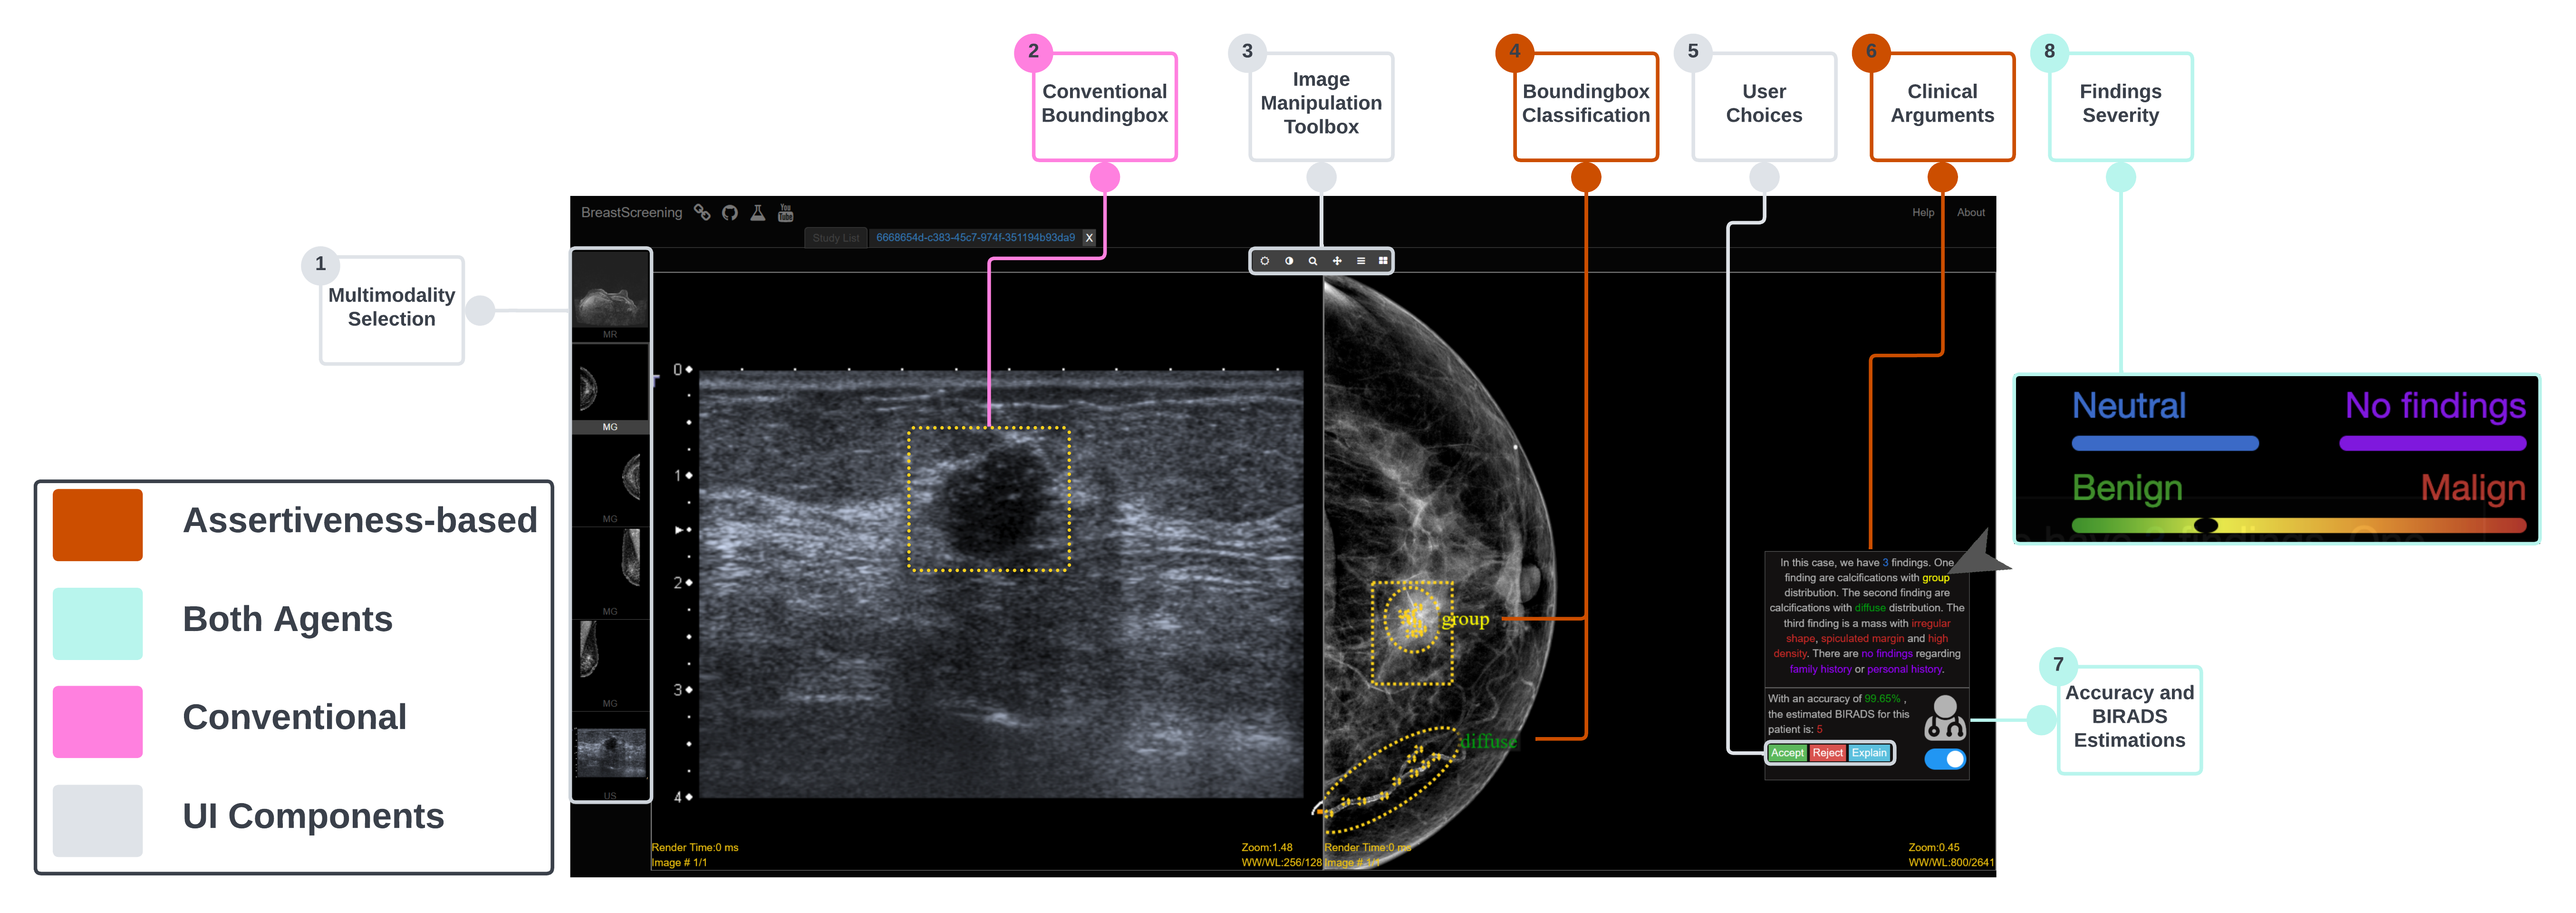
\includegraphics[width=1.000\textwidth]{fig096}
\caption[]{Interface for conventional and assertiveness-based AI agents for medical imaging analysis. Attributes are associated with numbers in each condition. AI agent provides severity information when hovering over variables. Colors range from benign (green) to malign (red). Number of findings displayed in neutral color (blue). Clinicians use purple color for family and personal history variables.}
\label{fig:fig096}
\end{figure}
%%%%%%%%%%%%%%%%%%%%%%%%%%%%%%%%%%%%%%%%%%%%%%%%%%%

Our assertiveness-based agent uses recommendations for classifying and segmenting:
(1) the number of detected findings;
(2) the patient severity of each breast and per medical imaging modality;
(3) a visual scale representing the benign or malign estimates;
(4) providing visualization of the sensitivity and specificity outcomes of the models; and
(5) with clinical arguments of the patient, such as pathological co-variables.
To compare the assertiveness-based agent to the conventional agent (Figure~\ref{fig:fig098}), we inform participants that the recommendations are generated by our \ac{AI} models so that they can also provide some feedback concerning the model performance.

Figure~\ref{fig:fig096} illustrates how the two \ac{AI} agents were integrated into an existing medical workflow for the classification of medical imaging data in support of breast cancer diagnosis.
Both agents are recommending classification and segmentation based on the DenseNet model~\cite{8721151} for \ac{MG} and \ac{US}, as well as based on the ResNet model~\cite{10.1145/3544548.3580682} for \ac{MRI}.
The two \ac{AI} agents provided the severity classification (Section~\ref{sec:app005009} of Appendix~\ref{chap:app005}) of the patient via \ac{BI-RADS}~\cite{SPAK2017179}, the accuracy of the model for that classification, and the segmentation of the lesion to explain the regions that derived from that classification.

\section{Research Questions \& Hypotheses}
\label{sec:chap006004}

The final purpose of our research is twofold.
Through assertiveness-based agents, we first aim to understand how personalized and customized communication could affect medical assessments in terms of the efficiency and efficacy of the clinical workflow.
Secondly, we aim to understand how clinicians perceive assertiveness-based agents differently.
Thus, our work addresses two primary research questions concerning the impact of assertiveness-based agents on efficiency and efficacy (RQ1), as well as the perception (RQ2) of clinicians.
We provide a more detailed view in Section~\ref{sec:app005005} of Chapter~\ref{chap:app005}.

\noindent
Specifically, we consider the following research questions and related hypotheses:

\vspace{0.5mm}

% New RQs
%%%%%%%%%%%%%%%%%%%%%%%%%%%%%%%%%%%%%%%%%%%%%%%%%%%
\begin{itemize}
\item {\bf RQ1.} How does an assertiveness-based agent affect medical assessments?
\begin{itemize}
\item {\bf H1.1.} Efficiency of clinicians in terms of time performance per each diagnosed patient will be higher with an assertiveness-based agent.
\item {\bf H1.2.} Classification accuracy of clinicians will not suffer with an assertiveness-based agent.
\item {\bf H1.3.} Through assertiveness-based communication, accuracy differences between novice and expert clinicians will depend on the tone of the personalized explanations.
\end{itemize}
\item {\bf RQ2.} How is an assertiveness-based agent perceived by clinicians?
\begin{itemize}
\item {\bf H2.1.} Clinicians will have a preference for an assertiveness-based agent.
\item {\bf H2.2.} Clinicians will consider an assertiveness-based agent more trustworthy.
\item {\bf H2.3.} Personalized highlights and explanations will not increase clinicians' workload nor decrease usability.
\item {\bf H2.4.} Novice and expert clinicians will perceive reliability and capability differently, depending on the levels of assertiveness.
\end{itemize}
\end{itemize}
%%%%%%%%%%%%%%%%%%%%%%%%%%%%%%%%%%%%%%%%%%%%%%%%%%%

In real-world clinical settings, clinicians' time is a limited and expensive resource that should be reallocated efficiently.
We take the position that while clinicians should make their clinical assessments with care, \ac{AI} agents can help with diagnosis efficiency.
Our assertiveness-based agent is designed to summarize the recommendations and to provide clinical arguments explaining the underlying classification and segmentation of the \ac{AI} models.

\section{Methods}
\label{sec:chap006005}

Our study aims to improve clinical decision-making by exploring personalized and customized mechanisms for adapting agent communication based on clinicians' medical experience.
More detailed methods are provided in Section~\ref{sec:app005006} of Appendix~\ref{chap:app005}.
We conducted 52 semi-structured interviews and user testing with clinicians to gather insights.
Our research involved a two-condition, within-subjects, counterbalanced experiment, with each participant taking part in three trials, providing valuable information for analysis.
Interviews were conducted between March 2022 and June 2022.
The research questions (Section~\ref{sec:chap006004}) emerged from these interviews and user-centered activities such as workshops, focus groups, and prototype co-design.
Participants included clinicians from various healthcare institutions, as well as researchers from the \ac{ML} and \ac{HCI} fields.
Ethical approval was obtained from the relevant clinical institutions.
In the following sections, we provide a detailed description of our controlled experiment, including the task, dataset, participant information, study procedures, and statistical analysis.

\subsection{Task}
\label{sec:chap006005001}

In our study, we focused on breast cancer diagnosis in imaging classification, a domain known for its high \ac{FP} rates.
We compared conventional and assertiveness-based agents in assisting trained medical personnel in this diagnostic task.
The conventional condition utilized the publicly available {\it BreastScreening-AI} framework (Section~\ref{sec:app005016})~\cite{CALISTO2022102285}, while we developed two additional conditions to personalize and customize \ac{AI} outcomes for clinicians (\href{https://mida-project.github.io/prototype-multi-modality-assistant/}{git.io/JMjDi}).
We conducted multiple trials with clinicians of different expertise levels, evaluating their interactions with the conventional, non-assertive, and assertive agents.
Clinicians diagnosed three patients with varying breast severities using different imaging modalities (Section~\ref{sec:app005010} of Appendix~\ref{chap:app005}), assessing the likelihood and location of the malignancy.
The task involved reading six imaging views per patient and classifying the severity using the \ac{BI-RADS} scale (Section~\ref{sec:app005014}).
A breast cancer diagnosis is challenging due to the diverse appearances of lesions, making accurate and consistent interpretation difficult for clinicians~\cite{CALISTO2022102285}.
Our study aimed to address this challenge and the associated error rates by exploring the use of \ac{AI} agents in medical imaging assessments.
Further details and analysis of our methods can be found in Section~\ref{sec:app005006001} of Appendix~\ref{chap:app005}.

\subsection{Dataset}
\label{sec:chap006005002}

In this work, we utilized a total of 338 cases from the \acs{HFF} clinical institution (Section~\ref{sec:app005006003} of Appendix~\ref{chap:app005}), with 289 cases classified by the head of radiology (Section~\ref{sec:app005006002}).
These cases included X-ray \acs{MG} images (\acs{CC} and \acs{MLO} views), \acs{US} images, and \acs{DCE-MRI} images.
For the \acs{MRI} volumes, multiple image slices containing the lesion were used.
This resulted in approximately 2890 images, which were used to train and test the \ac{AI} models.
To prepare the data for the models (Section~\ref{sec:app005012}), we performed pre-processing techniques, including data normalization, resizing the images to 224x224 pixels, and normalizing the images by subtracting the mean and dividing by the \acs{SD} (Section~\ref{sec:app005013}).
For more detailed information on the used dataset, please refer to Section~\ref{sec:app005006002} of Appendix~\ref{chap:app005}.

\subsection{Participants}
\label{sec:chap006005003}

We recruited 52 clinicians from various clinical environments (Section~\ref{sec:app005011}), including public hospitals, cancer institutes, and private clinics, to participate in our study.
For more detailed information on participants, please refer to Section~\ref{sec:app005006003} of Appendix~\ref{chap:app005}.
The clinicians were recruited from 11 different clinical institutions, and all participants provided their voluntary consent to use their data for research purposes.
The participants included a mix of expert clinicians (55.77\%), seniors with over 10 years of experience (34.62\%), middle clinicians with 5 to 10 years of experience (21.15\%), novice clinicians (44.23\%), juniors with up to 5 years of experience (32.69\%), and interns (11.54\%).
Each clinician was exposed to the three trials (conventional, assertive, and non-assertive) in a counter-balanced manner.

\subsection{Procedure}
\label{sec:chap006005004}

In this section, we provide an overview of the procedure followed in our study.
However, detailed information about the procedure will be described in Section~\ref{sec:app005006004} of Appendix~\ref{chap:app005}.
The procedure involved obtaining informed consent from the participants and collecting demographic information.
Clinicians familiarized themselves with the user interface and fundamental functionalities of the \ac{AI} agents before interacting with them in two different conditions: conventional and assertiveness-based.
Each clinician diagnosed three patients, once with the conventional condition and twice with the assertiveness-based conditions, divided into assertive and non-assertive trials in the last.
After each task, clinicians provided feedback on their perception of each \ac{AI} agent, including dimensions of trust, cognitive workload, and usability.
Preferences and ratings of assertiveness levels were also measured.

\subsection{Analysis}
\label{sec:chap006005005}

In this work, we analyzed to investigate the impact of the assertiveness-based agent on clinicians' efficiency, efficacy, and perceptions (Section~\ref{sec:app005006005} of Appendix~\ref{chap:app005}).
For {\bf RQ1}, we compared the time performance and accuracy of clinicians using one-way \ac{ANOVA} tests and examined the relationship between expertise and assertiveness levels.
For {\bf RQ2}, we compared clinicians' preferences, trustworthiness, cognitive workload, and usability ratings using \ac{ANOVA} tests.
Additionally, we conducted a qualitative analysis to identify emerging themes and inform customization of \ac{AI} recommendations.
The detailed analysis description will be presented in Section~\ref{sec:app005006005} of Appendix~\ref{chap:app005}.

\section{Results}
\label{sec:chap006006}

In this section, we summarize the results obtained from our study.
This section serves as an overview of the key findings, which will be further detailed in Section~\ref{sec:app005007} of Appendix~\ref{chap:app005}.
To analyze our hypotheses, we conducted a one-way \ac{ANOVA} test using the \texttt{scipy} library in Python, with medical professional experience as the main factor.
We focused on statistically significant results and selectively reported them, following recommendations from the literature~\cite{CASALE2022107302}.
Our analysis explored various aspects, including time performance, accuracy, decision rates, preference choices, agreement comparisons, and perceptions of reliability and capability.
Further details of the results, including figures and tables depicting the findings, can be found in Section~\ref{sec:app005007} of Appendix~\ref{chap:app005}.
This section provides a comprehensive and in-depth exploration of the data, allowing for a thorough understanding of the implications of our study.

\subsection{RQ1: Impact of an Assertiveness-Based Agent on Medical Assessments}
\label{sec:chap006006001}

This section summarizes our results to answer question {\bf RQ1}.
Specifically, the assertiveness-based agent had a positive impact on clinicians' time performance without compromising accuracy.
The agent's communication tone could be personalized based on the clinicians' expertise level, and the assertiveness-based condition showed advantages in decision-making.
The detailed outcomes and analysis can be found in Section~\ref{sec:app005007001} of Appendix~\ref{chap:app005}.

The impact of an assertiveness-based agent on medical assessments was investigated in this section.
We hypothesized that assertive communication between clinicians and the intelligent agent would alter clinicians' workflow and improve their time performance ({\bf H1.1}).
The results confirmed this hypothesis, as the time performance of clinicians improved significantly when using the assertiveness-based agent compared to the conventional agent (Figure~\ref{fig:fig099} on Section~\ref{sec:app005007001} of Appendix~\ref{chap:app005}).
The difference was statistically significant (F = 11.32, p = 0.005 $<$ 0.05), indicating a large effect size (r = 0.49).

Additionally, we hypothesized that the assertiveness-based agent would not impact the accuracy of clinicians (\textbf{H1.2}).
The results showed any significance (F = 1.85, p = 0.37 $>$ 0.05) in accuracy between the assertiveness-based agent and the conventional agent (Figure~\ref{fig:fig084}).
This supports our hypothesis that clinicians' accuracy in classifying patients was not negatively affected by assertiveness-based explanations.
Table~\ref{tab:tab018} provides summarized insights into the acceptance and rejection rates of \ac{AI} recommendations by clinicians.
For more detailed results, please refer to Table~\ref{tab:tab014} on Section~\ref{sec:app005007001}.

%%%%%%%%%%%%%%%%%%%%%%%%%%%%%%%%%%%%%%%%%%%%%%%%%%%
\begin{table}[htpb]
\centering
\begin{tabular}{|c|cc|ll|}
\hline
\multirow{2}{*}{\textbf{Trials}} & \multicolumn{2}{c|}{\textbf{Overall Corrects}} & \multicolumn{2}{c|}{\textbf{Overall Mistakes}} \\ \cline{2-5} 
                & \multicolumn{1}{c|}{\textbf{Novice}}         & \multicolumn{1}{c|}{\textbf{Expert}}        & \multicolumn{1}{c|}{\textbf{Novice}}         & \multicolumn{1}{c|}{\textbf{Expert}}        \\ \hline
\textbf{Conventional}        & \multicolumn{1}{c|}{{\color[HTML]{9A0000} 69.70\%}}       & {\color[HTML]{9A0000} 63.77\%}      & \multicolumn{1}{l|}{{\color[HTML]{9A0000} 30.30\%}}       & {\color[HTML]{9A0000} 36.23\%}      \\ \hline
\textbf{Assertive}           & \multicolumn{1}{c|}{{\color[HTML]{009901} 81.59\%}}       & 65.76\%      & \multicolumn{1}{l|}{{\color[HTML]{009901} 18.41\%}}       & 34.25\%      \\ \hline
\textbf{Non-Assertive}       & \multicolumn{1}{c|}{75.63\%}       & {\color[HTML]{009901} 66.41\%}      & \multicolumn{1}{l|}{24.37\%}       & {\color[HTML]{009901} 33.59\%}      \\ \hline
\end{tabular}%
\caption{Percentage of clinicians' acceptance/rejection of \acs{AI} recommendations. Shows how often clinicians switched conclusions after interacting. ``Overall Corrects'' indicates correct acceptance/rejection. ``Overall Mistakes'' denotes incorrect acceptance/rejection.}
\label{tab:tab018}
\end{table}
%%%%%%%%%%%%%%%%%%%%%%%%%%%%%%%%%%%%%%%%%%%%%%%%%%%

Furthermore, we examined the impact of personalized explanations by customizing the agent's communication for novice and expert clinicians (\textbf{H1.3}).
The results revealed a significant association ($\chi^2$ = 3.84, p = 0.001 $<$ 0.05) between the agent's communication tone and medical professional experience.
Novice clinicians had a higher chance of correctly classifying a patient with the assertive agent, while expert clinicians had a slightly higher chance with the non-assertive agent.
These findings suggest tailoring the agent's assertiveness to the clinician's experience level.

The analysis also compared switching decision rates between the assertiveness-based and conventional agents.
The results showed that clinicians made better decisions with assertiveness-based assistance, resulting in higher correct acceptance and rejection rates than the conventional condition.
This highlights the importance of scenario design in evaluating clinicians' performance.

\subsection{RQ2: Perception of Clinicians towards an Assertiveness-Based Agent}
\label{sec:chap006006002}

In this section, we provide a summarized overview of our investigation into question {\bf RQ2}.
However, for a more comprehensive understanding of our research findings, we present a detailed analysis in Section~\ref{sec:app005007002} of Appendix~\ref{chap:app005}.
Our analysis provides a comprehensive understanding of how clinicians perceive and interact with \ac{AI} technology in the context of medical assessments.

Gathering feedback and perspectives from clinicians allowed us to gain valuable insights into their experiences and attitudes toward these agents.
The results (Figure~\ref{fig:fig085}) showed a significant preference (F = 8.35, p = 0.001 $<$ 0.05) for the assertiveness-based agent ({\bf H2.1}), with 66\% of participants favoring it.
At the same time, 24\% expressed a preference for the conventional agent, and 10\% had no specific preference.
This highlights the importance of considering clinicians' preferences and the potential benefits of incorporating assertiveness-based communication in medical decision-making processes.

%%%%%%%%%%%%%%%%%%%%%%%%%%%%%%%%%%%%%%%%%%%%%%%%%%%
\begin{figure}[htpb]
\centering
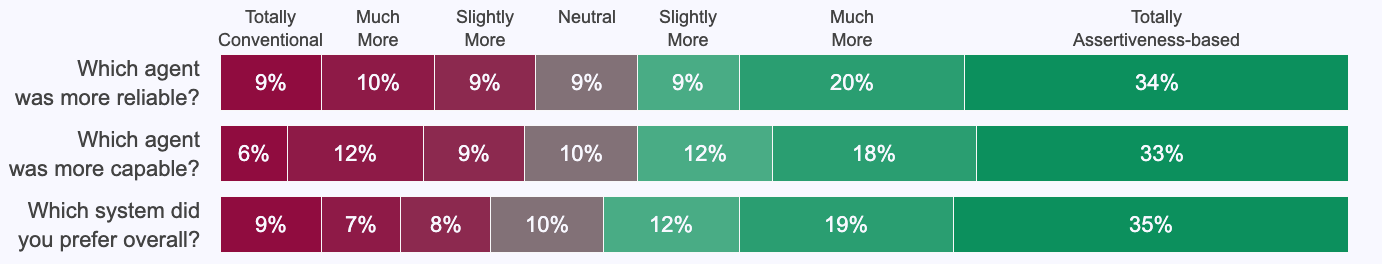
\includegraphics[width=1.000\textwidth]{fig085}
\caption[]{Preference choices of clinicians when comparing both conventional and assertiveness-based agents within this study. Rates of clinicians are ranging from {\it Totally Conventional} to {\it Totally Assertiveness-based} on perceived {\it reliability}, {\it capability}, and {\it overall preference} of each agent.}
\label{fig:fig085}
\end{figure}
%%%%%%%%%%%%%%%%%%%%%%%%%%%%%%%%%%%%%%%%%%%%%%%%%%%

Clinicians' perceptions of trust, understanding, competence, and thoughtfulness towards the conventional and assertiveness-based agents were examined (Table~\ref{tab:tab013} on Section~\ref{sec:app005007002}).
The results indicated comparable trustworthiness (F = 19.47, p = 0.06 $>$ 0.05) between the agents.
No significant differences (p = 0.14 $>$ 0.05) in understanding were found.
The assertiveness-based agent was perceived as more competent (p = 0.04 $<$ 0.05), and clinicians showed higher thoughtfulness with this agent (p = 0.001 $<$ 0.05).
These findings partially support our hypothesis ({\bf H2.2.}) on preference choices.

We assessed the workload and usability of the conventional and assertiveness-based agents and found no significant differences.
There were no significant differences in the workload scores measured by the \ac{NASA-TLX} (p = 0.38 $>$ 0.05) and no significant differences in the usability scores measured by the \ac{SUS} (p = 0.38 $>$ 0.05).
These results support our hypothesis ({\bf H2.3.}) that personalization will not increase clinicians' workload nor decrease usability, with no significant differences between agents.

Last, we examined how clinicians perceive the levels of assertiveness in communicating clinical arguments (Figure~\ref{fig:fig091} on Section~\ref{sec:app005007002} of Appendix~\ref{chap:app005}).
The results revealed significant differences in reliability (F = 31.36, p = 0.0001 $<$ 0.05) and capability (F = 18.17, p = 0.0003 $<$ 0.05) between novice and expert clinicians.
These findings support our hypothesis ({\bf H2.4.}) that clinicians' preferences vary based on the assertiveness level of the agent, indicating differing perceptions of clinical arguments.

\subsection{Summarized Qualitative Insights}
\label{sec:chap006006003}

This section provides a summarized overview of the qualitative analysis of clinicians' perceptions and experiences with conventional and assertiveness-based agents.
For a more detailed analysis, refer to Section~\ref{sec:app005007003} of Appendix~\ref{chap:app005}.
We used a participatory approach to analyze the data collected from focus group sessions, participant opinions, and transcripts.
Through emergent affinity diagrams, common themes were identified regarding clinicians' perceptions of clinical arguments and visualizations of \ac{AI} recommendations.
This qualitative analysis yielded valuable insights into the impact of assertiveness-based agents on clinicians' workflows and mental models.

The qualitative findings revealed that clinicians overwhelmingly preferred human-interpretable arguments over numeric representations of \ac{AI} output classifications (Section~\ref{sec:app005007003001} of Appendix~\ref{chap:app005}).
In fact, 92\% of clinicians preferred the personalized communication and clinical arguments provided by the assertiveness-based agent over the conventional agent.
They found that the assertiveness-based agent enhanced their decision-making process by providing more meaningful and understandable explanations for the \ac{AI} recommendations.
One junior clinician stated, ``{\it The assertiveness-based gave me a better understanding of the AI's reasoning, which helped me make more informed decisions}'' (C6).

Our qualitative insights provided evidence of how clinicians develop mental models of \ac{AI} agents based on their preconceived notions and comparative experiences (Section~\ref{sec:app005007003002} of Appendix~\ref{chap:app005}).
A clinician described the difference, saying, ``{\it The first AI [assertiveness-based] was outstanding... but in the second AI [conventional] I was frustrated with the lack of communication in comparison to the first one}'' (C48).
Expert clinicians used the communication tone to anticipate wrong \ac{AI} recommendations, while novice clinicians focused on the learning process and patient comparisons.
These observations highlight the importance of personalized and customized communication to cater to the varying needs and expectations of clinicians.
These findings contribute to the growing understanding of the impact of \ac{AI} communication on clinicians' decision-making processes and highlight the importance of designing \ac{AI} systems with user-centered approaches~\cite{10.1145/3491102.3517789}.
Something that was indicated in Chapter~\ref{chap:chap005}.

\section{Discussion}
\label{sec:chap006007}

In this section, we provide a condensed overview of the in-depth discussion presented in Section~\ref{sec:app005008} of Appendix~\ref{chap:app005}, where we explore the insights derived from our study and offer targeted recommendations for designing and integrating intelligent agents into the field of medical imaging.
We studied how personalized and customized communication of an intelligent agent can aid clinicians in their decision-making during medical imaging diagnosis.
We conducted a within-subject to investigate how clinicians perceive assertiveness-based agents differently.
Our results show that assertiveness-based agents can alter clinicians' workflows by increasing the efficiency of clinicians while maintaining overall efficacy.

Our findings revealed that the classification accuracy was unaffected by assertiveness-based communication.
However, the tone of the explanations had a significant influence on the decision-making behavior of novice and expert clinicians.
This emphasizes the need for compliant agents that provide personalized and tailored explanations.
By addressing this, future developments can focus on enhancing the provision of relevant and customized explanations, ultimately improving the effectiveness of intelligent agents in medical imaging diagnosis.
These insights contribute to healthcare, \ac{HCI}, decision support, and \ac{AI} communication research.

\subsection{Design Implications}
\label{sec:chap006007001}

This section explores valuable design implications for developing innovative \ac{AI} systems in the clinical domain.
It covers various topics such as combining diverse knowledge classifiers (Section~\ref{sec:app005008001001}), enriching training models with additional information (Section~\ref{sec:app005008001002}), and designing intuitive and user-friendly \acp{UI} for effective agent communication (Section~\ref{sec:app005008001003}).
The generalizability and broader applicability of the study to other related fields are also discussed (Section~\ref{sec:app005008001004}).
Further in-depth insights and recommendations can be found in Section~\ref{sec:app005008001} of Appendix~\ref{chap:app005}.

Including lesion details and the relevance of classification is crucial for improving decision-making in breast cancer diagnosis (Section~\ref{sec:app005008001001}).
By aligning the \ac{AI} system with clinicians' mental models and providing personalized guidance and explanations, intelligent agents can enhance clinicians' decision-making.
Future research should focus on training models with mixed information to effectively integrate them into clinical workflows.
These insights and recommendations contribute to developing human-centered and efficient medical \ac{AI} systems, ultimately improving clinical outcomes and patient care.

The study suggests that personalization of agent communication can positively impact clinical workflows and trust.
To achieve this, \ac{DL} models must predict mixed clinical arguments and adapt communication based on clinicians' experience and demographics (Section~\ref{sec:app005008001002}).
This approach can be implemented through fused training or separate models for each variable.
Personalizing agent communication and incorporating patient information improves intelligent agents in medical imaging, benefiting decision-making and patient outcomes.

The focus is on evaluating personalized and customized communication between agents and clinicians with different medical experience levels (Section~\ref{sec:app005008001003}), specifically by adapting the communication tone.
While the results suggest its potential effectiveness, future research should explore other clinicians' demographic characteristics or agent behaviors to enhance decision-making (Section~\ref{sec:app005015}).
Qualitative findings indicate clinicians' willingness to adjust communication based on the \ac{AI}'s confidence, a warranting investigation into the impact of different performance actions on decision-making.
In conclusion, this section expands on personalized communication in medical \ac{AI} and emphasizes its potential benefits, considering clinicians' experience and confidence in improving care outcomes.

While caution is needed when generalizing the study's findings to other medical domains (Section~\ref{sec:app005008001004}), the personalized and customized communication techniques identified can benefit various medical diagnoses, considering shared challenges across specialties.
For instance, lung cancer and skin cancer diagnosis could also benefit from tailored agent communication, matching clinicians' expertise and background, resulting in improved accuracy and patient outcomes.
Moreover, studies supporting personalized medicine in \ac{AI}-based systems for diagnosis and treatment guidance further validate the relevance and potential impact of the recommendations beyond assertiveness-based agents.

\subsection{Limitations}
\label{sec:chap006007002}

This section summarizes the analysis of the study constraints discussed in Section~\ref{sec:app005008002} of Appendix~\ref{chap:app005}.
The study on assertiveness-based agents in breast cancer diagnosis faced challenges due to limited clinician availability and remote study conditions, impacting task control and clinician interactions.
Liability implications in medical settings and evolving legal frameworks present further limitations, requiring research and legal developments.
Future efforts should focus on robust frameworks and guidelines to address risks and establish accountability.
Training personalized \ac{DL} models and exploring different agent features are areas for future exploration.

\section{Conclusion}
\label{sec:chap006008}

In this work, we provide a novel perspective on how to personalize and customize the explanations of intelligent agents to human clinicians.
Our results from an experimental study with 52 clinicians comparing a conventional agent to an assertiveness-based agent suggest that the ability of a system to not only exploring how to adapt the communication tone ({\it i.e.}, more suggestive or more assertive), but also provide granular explanations of patient cases has merits for end users.
From our results, the time performance was satisfactory, where clinicians took less 25\% of the time to diagnose a patient with the assertiveness-based agent in comparison to the conventional agent.
As we observed, the caparison between the conventional agent and the assertiveness-based agent was more effective also with the latter in achieving the proper diagnostic of the patient.
Additionally, our results demonstrate that if explanations are adapted taking into account the medical experience of clinicians, accuracy chance of correctly diagnosing a patient is 91\% higher for novice and 78\% higher for expert clinicians.
Last, clinicians are showing an increase in trust, preferring the assertiveness-based agent by being more reliable and capable, as this agent was revealing to be further understandable, competent and thoughtful.
Our work has implications for the design of \ac{AI} systems not only in the medical domains, but also in fields that are facing similar challenges, demanding a personalization of the human-AI interaction.